\section{Introduction}
\subsection{Previous work}
Current research started as part of the studies on the Mathematics Expert in
Data Analytics and Machine Learning postgraduate specialization program \cite{_ai&ml_}
held by the AI Research Group of Eötvös Lóránd University \cite{_ai_}.
During the one-year program a thesis work has to be created that is often
preceded by a modeling practice in the first semester.
This project follows the same approach as railway track fault detection models
were already built in the first semester.
However, the characteristics of the dataset used at that time did not allow a
successful application of a model however valuable experience is gained together
with a boost of motivation to follow up the topic and deepen the knowledge in the
mentioned problem.

\subsection{Available results}
The work of the first semester can be found at \cite{tomcom_mathemathical_2022}.
Following is a short summary of the results obtained.

During the first semester basic convolutional neural networks were built with a classification
head to identify images with defective railway tracks.
LeNet-5, AlexNet, VGG16 and ResNet50 were applied, partially utilizing transfer learning as well
(indicated with \lstinline{*_p} in the following Figures).

The dataset was taken from the Kaggle webpage \cite{_railway_} consisting of a limited
number of images with defective and non-defective railway tracks.
The images combine a high variety of failures with very limited examples leading to a very
specific dataset where the provided validation and test split is not representing the initial
set of images.

The results of the modeling is shown on Figure \ref{fig:Kaggle_results}, where the performance of
different bootstrapped models on the splits of the dataset is given.

\begin{figure}[!ht]
    \centering
    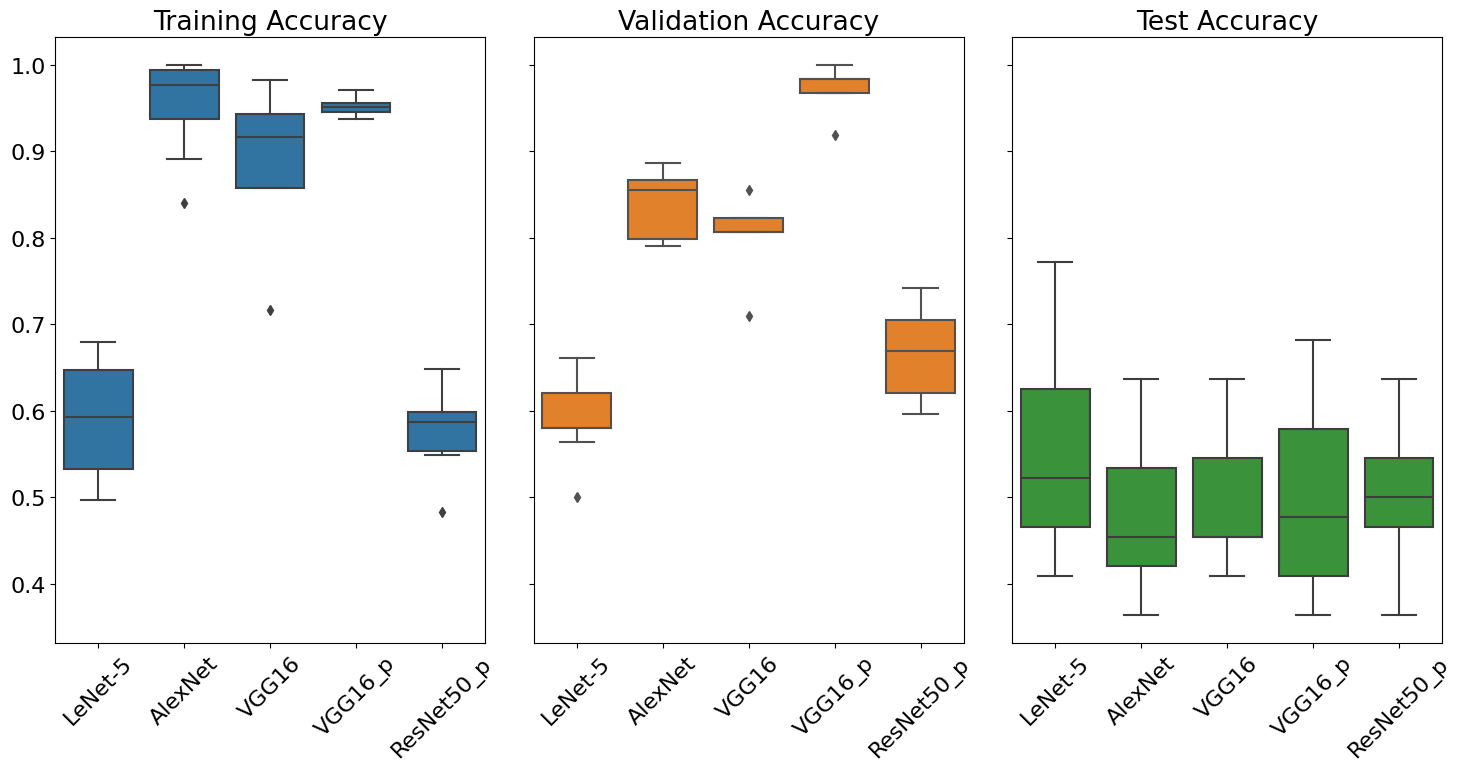
\includegraphics[width=\textwidth]{./tex_images/bootstrap_results.png}
    \caption{Results of first classification approach on the Kaggle dataset}
    \label{fig:Kaggle_results}
\end{figure}

Most of the models were successfully learned the features of the training and validation datasets,
however on the test dataset all failed to classify the images in an acceptable level, mostly
achieving the level of a random classifier only.
This lead to the realization that the low number of images compared with the high variety of the track
failures will result in a situation where the model can easily learn the specifics of the training and
validation dataset preventing of any generalization to the test dataset.

As a followup a search for a more extended dataset and more refined models were started.

\subsection{MÁV CRTI Ltd.}

The company MÁV Central Rail And Track Inspection Ltd. (MÁV CRTI Ltd.) \cite{_mav_} was approached
as they are proficient in railway track inspection and have the equipment and data that could be used
for building such classifier model.

The MÁV CRTI Ltd. was established in 1996 by MÁV Hungarian State Railways Co.
The scope of the company covers the fields of technical inspection and analysis related
railway tracks, rails and corresponding structures:
\begin{itemize}
    \item Geometric measurement of tracks and geometric condition survey
    \item Measurement, examination and qualification of railway rails
    \item Qualification of new and used superstructure materials
    \item Examination of bridges
    \item Examination of substructures
    \item Development related to rail measurement, examination and line maintenance
\end{itemize}

A comprehensive overview about the company, it's activities and history can be found at
\cite{_mav_} and in \cite{kfv_25years}.

The Rail Diagnostic Department carries out regular measurements on the railway tracks in order
to determine the overall condition of the rails and thus ensuring the safety of railway operation.
These inspections are carried out by special railway measurement equipment and inspection vehicles,
Starting from the simplest visual inspections carried out by the maintenance personnel up to
special ultrasonic examinations and rail profile measurements.
With such equipment rail surface and internal defects can be detected and detailed information about
the track profile can be obtained along hundreds of kilometers of railway tracks.

The Rail Diagnostic Department already has some experience with machine learning based rail
defect detection providing options for benchmarking the models created through this project.
It also reflects the importance of such approach, as today visual inspection demands heavy efforts
let that be the work done by the maintenance personnel (intrinsically walking along the tracks)
or the monitoring of the video footage taken during the inspection rides.

Currently, MÁV CRTI Ltd. operates two vehicles for rail inspection purposes, the SDS and FMK-008 shown on
Figure \ref{fig:vehicles}, both equipped with different measurement and inspection systems.
Fortunately both of them is equipped with video recording, however with different systems.
After a first view on the video files the system of the SDS vehicle is selected for a first modelling
approach.

\begin{figure}[!ht]
    \centering
    \begin{subfigure}{0.45\textwidth}
        \centering
        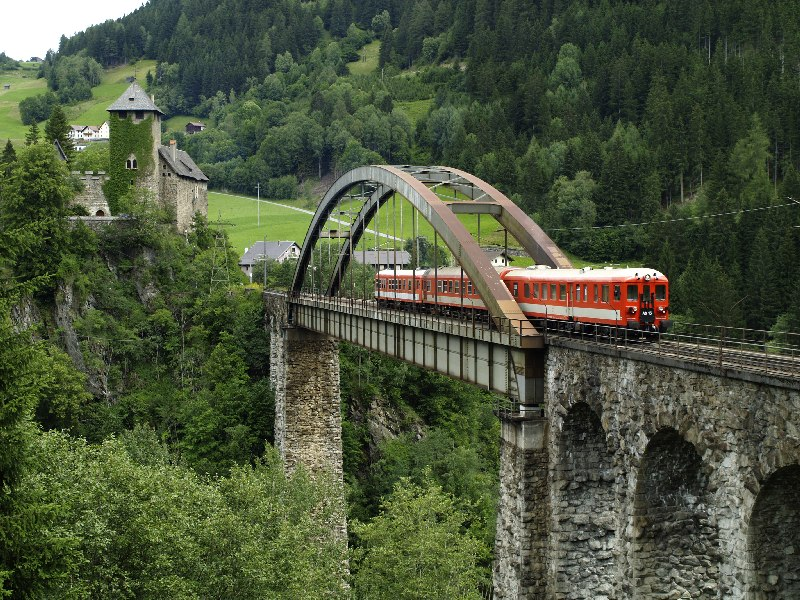
\includegraphics[height=3cm]{./tex_images/sds.jpg}
        \caption*{SDS}
    \end{subfigure}
    \begin{subfigure}{0.45\textwidth}
        \centering
        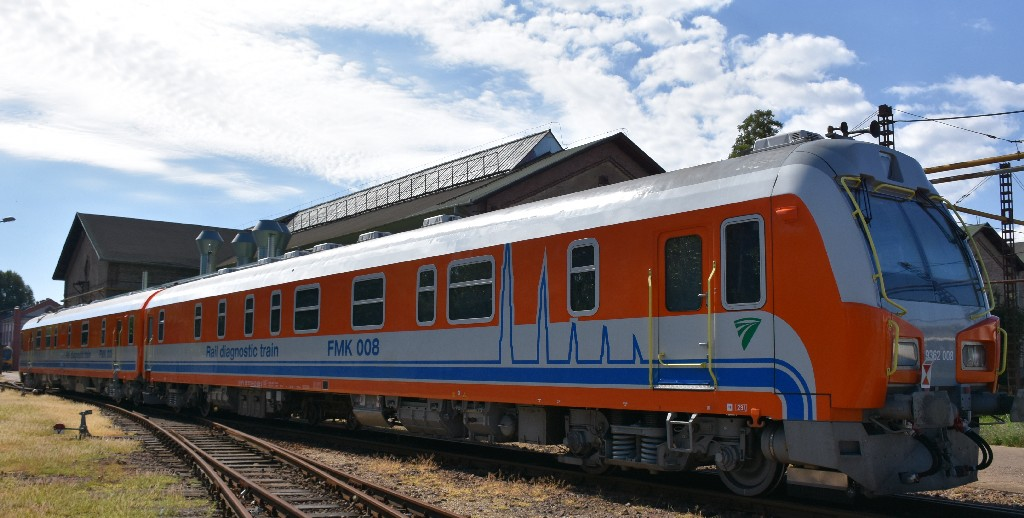
\includegraphics[height=3cm]{./tex_images/FMK008.jpg}
        \caption*{FMK-008}
    \end{subfigure}
    \caption{Railway inspection vehicles of MÁV CRTI Ltd.}
    \label{fig:vehicles}
\end{figure}

\subsection{Modeling approach and problem statement}
During the first part of the project convolutional neural networks with classification head were applied
on annotated dataset.
A step forward was taken by obtaining real world data, however this comes with the burden of
missing labeling.
Therefore, the modeling approach was also changed from supervised learning to unsupervised learning.
In this way the problem was reformulated and traced back to anomaly detection, thus resulting in the
following key questions:

\begin{enumerate}[label=Q\arabic*]
    \item \label{itm:Q1} Can anomaly detection algorithms used to detect rail defects?
    \item \label{itm:Q2} What models could be applied on the given dataset?
    \item \label{itm:Q3} What accuracy rate can be achieved with the models?
\end{enumerate}

\subsection{Structure of the document}
The Section \ref{dataset} gives a deep view on the sample dataset.
The structure of the models introduced in Section \ref{model}.
The realization of the models, structure of the software code is explained in Section \ref{sw_code}.
The results are interpreted in Section \ref{results} and discussed in Section \ref{discussion}.
Further steps and possible improvement options covered with a summary of the results in \ref{conclusion}.